\documentclass[10pt,handout]{beamer}

\usetheme{metropolis}
\usepackage{appendixnumberbeamer,amsmath}
\usepackage[ruled,vlined]{algorithm2e}
\usepackage{booktabs}
\usepackage[scale=2]{ccicons}
\usepackage{tikz}
\usetikzlibrary{arrows.meta,positioning,calc,decorations.pathreplacing}

\DeclareMathOperator{\order}{Order}

\usepackage{libertine}
\usepackage[libertine]{newtxmath}
\usepackage{mathrsfs}
\include{../../letterfonts}
\DeclareMathOperator{\enc}{Enc}
\DeclareMathOperator{\res}{Res}
\DeclareMathOperator{\spec}{Spec}
\DeclareMathOperator{\cov}{Cov}
\DeclareMathOperator{\Var}{Var}
\DeclareMathOperator{\Rank}{rank}
\newcommand{\Tfae}{The following are equivalent:}
\newcommand{\tfae}{the following are equivalent:}
\newcommand{\sparsity}{\textit{sparsity}}
\DeclareMathOperator{\poly}{poly}
\newtheorem{claim}{Claim}
\title{Nisan's Pseudorandom Generator for \textsf{RL}}
\subtitle{$\textsf{BPL}\subseteq \textsf{SC}=\textsf{DTISP}(\poly(n),\log^2(n))$}
\date{December 2, 2025}
\author{Soham Chatterjee}
\institute{Pesudorandomness Course (CSS.413.1) Presentation, STCS}
\metroset{block=fill}
\pagestyle{empty}
\begin{document}

\maketitle

% \begin{frame}{Table of contents}
% 	\setbeamertemplate{section in toc}[sections numbered]
% 	\tableofcontents[hideallsubsections]
% \end{frame}
\begin{frame}{Complexity Classes}
	\begin{itemize}
		\item \textcolor{blue}{\textsf{L}}: Deterministic Logarithmic Space.
		\item $\mathcolor{blue}{\mathsf{L}^\alpha}$, $\mathcolor{blue}{\alpha> 0}$: Set of problems decidable in $\mathcolor{blue}{O(\log^{\alpha}n)}$ space deterministically.
		\item \textcolor{blue}{\textsf{NL}}: Nondeterministic Logarithmic Space.
		\item \textcolor{blue}{\textsf{RL}}: Randomized Logarithmic Space with One-sided error $\mathcolor{blue}{\frac13}$. 
		\item \textcolor{blue}{\textsf{BPL}}: Randomized Logarithmic Space with Two-sided error $\mathcolor{blue}{\frac13}$.
		\item \textcolor{blue}{\textsf{SC}}: Steve's Class or \textcolor{blue}{\textsf{DTISP}}$\mathcolor{blue}{(\poly(n),\poly(\log n))}$ i.e. set of problems decidable deterministically in polynomial time and polylog space.
		\item \textcolor{blue}{\textsf{NC}}: Nick's Class i.e. set of problems decidable in circuits of polynomial size and polylog depth and bounded fan-in. 
	\end{itemize}
	\begin{alertblock}{Remark}
		Don't confuse \textcolor{blue}{\textsf{SC}} with $\mathcolor{blue}{\mathsf{P}\cap \textsf{PolylogSpace}}$!
	\end{alertblock}
\end{frame}
\begin{frame}[c]{Complexity Classes Zoo}

	\centering
	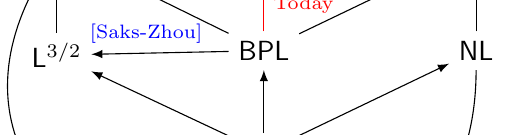
\begin{tikzpicture}[
			node distance=0.8cm and 2cm,
			class/.style={font=\sffamily},
			arrow/.style={-latex},
			annotation/.style={font=\scriptsize, text=blue}
		]
		\path[use as bounding box] (-3,-2) rectangle (3,-1);
		\node[class] (SC) at (0,0) {SC};
		\node[class, right=of SC] (NC) {NC};
		\node[class, left=of SC] (L2) {$\mathsf{L}^2$};

		% Now position other nodes relative to these
		\node[class, above=of NC] (P) {P};
		\node[class, above=of L2] (PolylogSpace) {PolylogSpace};
		\node[class, below=of SC] (BPL) {BPL};
		\node[class, below=of NC] (NL) {NL};
		\node[class, below=of L2] (L32) {$\mathsf{L}^{3/2}$};
		\node[class, below=of BPL] (RL) {RL};
		\node[class, below=of RL] (L) {L};

		% Draw arrows
		\draw[arrow] (L) -- (RL);
		\draw[arrow] (RL) -- (NL);
		\draw[arrow] (RL) -- (BPL);
		\draw[arrow] (RL) -- (L32);

		% From NL
		\draw[arrow] (NL) -- (NC);
		\draw[arrow] (NL) to[out=270,in=240,looseness=2.1] node[pos=0.7,annotation,above,sloped] {[Savitch]} (L2);

		% From BPL
		\draw[arrow] (BPL) -- (NC);
		\draw[arrow] (BPL) -- (L2);
		\draw[arrow] (BPL) -- node[midway,annotation,pos=0.6,above] {[Saks-Zhou]} (L32);

		% Left column
		\draw[arrow] (L32) -- (L2);
		\draw[arrow] (L2) -- (PolylogSpace);

		% From SC
		\draw[arrow] (SC) -- (PolylogSpace);
		\draw[arrow] (SC) -- (P);

		% From NC
		\draw[arrow] (NC) -- (P);
		% \draw[arrow, red] (BPL) -- node[midway,font=\scriptsize,right,pos=0.6,color=red] {Today} (SC);
		% \draw<1>[arrow] (BPL) -- (SC);

		% Red "Today" edge: appears starting slide 2
		\draw<2->[arrow, red] (BPL) --
		node[midway,font=\scriptsize,right,pos=0.6,color=red,align=left] {[Nisan]\\ Today} (SC);
	\end{tikzpicture}
\end{frame}
\begin{frame}{Pseudorandom Generator}
	\begin{definition}[Pseudorandom Generator]
		A map $\mathcolor{blue}{\mcG:\{0,1\}^l\to \{0,1\}^n}$, where $\mathcolor{blue}{n\geq l}$ is called a PRG for a class $\mathcolor{blue}{\mcC}$ with a parameter $\mathcolor{blue}{\epsilon>0}$ if for any $\mathcolor{blue}{f\in \mcC}$, $$\mathcolor{blue}{\left|\underset{y\in\{0,1\}^n}{\bbP}[f(y)=1]-\underset{x\in\{0,1\}^l}{\bbP}[f(\mcG(x))=1]\right|\leq \epsilon}$$
	\end{definition}
	\begin{itemize}
		\item Here $\mathcolor{blue}{l}$ is called the \textcolor{blue}{seed-length} of the PRG.
		\item $\mathcolor{blue}{n-l}$ is called the \textcolor{blue}{stretch} of the PRG.\pause
		\item We call $\mathcolor{blue}{\mcG}$, $\mathcolor{blue}{\epsilon}$-fools $\mathcolor{blue}{\mcC}$.\pause
		\item Typically, we want $\mathcolor{blue}{n>> l}$ and $\mathcolor{blue}{\mcG}$ to be efficiently computable.
	\end{itemize}
\end{frame}
\begin{frame}{Finite State Automata}
	Let $\mathcolor{blue}{T}$ be a \textsf{BPL} machine which uses $\mathcolor{blue}{n^c}$ random bits on inputs of length $n$ and runs in polynomial time and uses $\mathcolor{blue}{S=O(\log n)}$ space. \pause
	\begin{itemize}
		\item There are at most  $\mathcolor{blue}{N:=2^{O(S)}=\poly(n)}$ configurations of $\mathcolor{blue}{T}$. \pause
		\item Each random bit is used to make a transition between two configurations. \pause
		\item The starting configuration is fixed for any input. \pause
		\item Input $\mathcolor{blue}{x}$ is accepted if $\mathcolor{blue}{T}$ reaches a state representing acceptance.
	\end{itemize} \pause

	Therefore the configuration graph of $\mathcolor{blue}{T}$ on input $\mathcolor{blue}{x}$ represents a finite state automata with $\mathcolor{blue}{N}$ states.
\end{frame}
\begin{frame}[c]{Computational Tableau of \textsf{BPL} machine}
	\begin{figure}
		\centering
		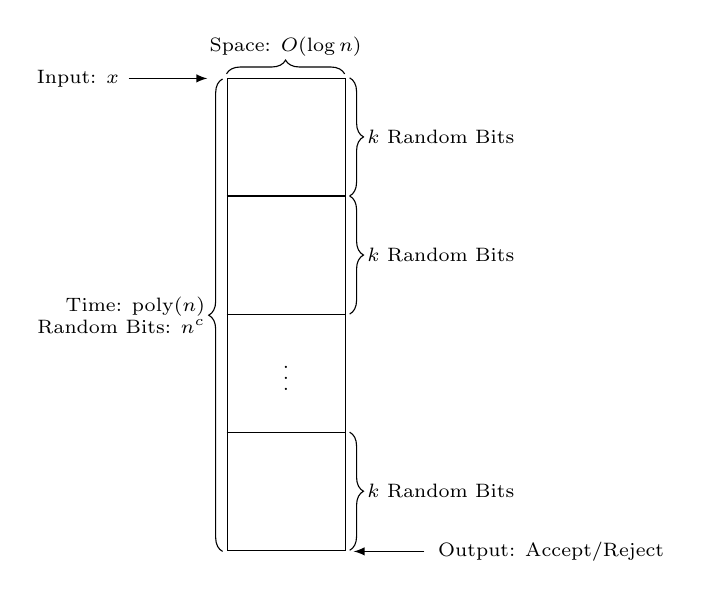
\begin{tikzpicture}[
				box/.style={draw, minimum width=1.5cm, minimum height=6cm},
				brace/.style={decorate,decoration={brace,amplitude=5pt}},
				arrow/.style={-latex},
				txt/.style={font=\scriptsize}
			]

			% Main box
			\node[box] (B) at (0,0) {};

			% Horizontal slices
			\draw (B.north west)++(0,-1.5) -- ++(1.5,0);
			\draw (B.north west)++(0,-3) -- ++(1.5,0);
			\draw (B.north west)++(0,-4.5) -- ++(1.5,0);

			% Left input arrow
			\draw[arrow] (-2,3) -- ++(+1,0);
			\node[txt, anchor=east] at (-2,3) {$\text{Input: } x$};

			% Right braces + text
			\draw[brace] (B.north east)++(+0.05,0) -- ++(0,-1.5)
			node[midway,right=0.1cm,txt] {$k$ Random Bits};

			\draw[brace] (B.north east)++(+0.05,-1.5) -- ++(0,-1.5)
			node[midway,right=0.1cm,txt] {$k$ Random Bits};

			\draw[brace] (B.north east)++(+0.05,-4.5) -- ++(0,-1.5)
			node[midway,right=0.1cm,txt] {$k$ Random Bits};
			% Left Brace + text
			\draw[brace]
			(B.south west)++(-0.05,0) -- ++(0,6)
			node[midway, txt, left=0.1cm, align=right]{Time: $\poly(n)$\\ Random Bits: $n^{c}$};
			% Top Brace + text
			\draw[brace] (B.north west) ++(0,0.05) -- node[txt,midway,above=0.1cm] {Space: $ O(\log n)$}++(+1.5,0);
			% Bottom output arrow
			\draw[arrow] (B.south east) ++ (+1,0) node[txt,right=0.05cm,align=left] {Output: Accept/Reject} -- ++(-0.9,0);

			% Annotations
			\node[txt] at (0,-0.7) {$\vdots$};
		\end{tikzpicture}
		\caption{Computational Tableau of \textsf{BPL} machine $T$.}
	\end{figure}

\end{frame}
\begin{frame}{Dividing \textsf{BPL} Computation into Blocks}
	\begin{itemize}
		\item Let the \textsf{BPL} machine $\mathcolor{blue}{T}$  run in time $\mathcolor{blue}{T(n)=\poly(n)}$  using $\mathcolor{blue}{n^{c}}$  random bits and $\mathcolor{blue}{O(\log n)}$  space on input $\mathcolor{blue}{x}$  of length $\mathcolor{blue}{n}$.\pause
		\item Let $\mathcolor{blue}{k<< n^{c}}$  be a parameter to be fixed later.
		\item Divide the computation of $\mathcolor{blue}{T}$  into $\mathcolor{blue}{t=n^c/k}$  blocks, where each block uses $\mathcolor{blue}{k}$  random bits.\pause
		\item We can treat each block as a separate \textsf{BPL} machine $\mathcolor{blue}{T_i}$  (in some sense) which takes input as the final configuration of $\mathcolor{blue}{T_{i-1}}$  and $\mathcolor{blue}{k}$  random bits.
	\end{itemize}
\end{frame}
\begin{frame}{FSA for Computation Blocks}
	\begin{itemize}
		\item We can think of $\mathcolor{blue}{T}$  as a finite state automata with $\mathcolor{blue}{N}$  states.
		\item Each state makes $\mathcolor{blue}{2^k}$  transitions where each transion corresponds to a choice of $\mathcolor{blue}{k}$  random bits. \pause
		\item Let $\mathcolor{blue}{Q}$  be this automata. For transition we write $\mathcolor{blue}{Q(i;r)=j}$  for any $\mathcolor{blue}{r\in\{0,1\}^k}$  if $\mathcolor{blue}{Q}$  goes from state $\mathcolor{blue}{i}$  to state $\mathcolor{blue}{j}$  when fed $\mathcolor{blue}{r}$. \pause
		\item Let $\mathcolor{blue}{M}$  be the matrix where $\mathcolor{blue}{M[i,j]=\underset{r\in\{0,1\}^k}{\bbP}[Q(i;r)=j]}$ \pause
	\end{itemize}
	$$\mathcolor{blue}{\underset{r\in \{0,1\}^{k\times t}}{\bbP}[T(x,r)=\text{Acc}]=\sum_{j:\text{Accepting state}}M^t[1,j]}$$


	\textbf{Goal:} Approximate $\mathcolor{blue}{M^t}$  using PRG.
\end{frame}
\begin{frame}{Approximate Automata Matrix}
	Suppose we have a pseudorandom generator $\mathcolor{blue}{\mcG:\{0,1\}^k\to \{0,1\}^{k\cdot t}}$. Let $\mathcolor{blue}{Q}$  be a finite state automata with $\mathcolor{blue}{N}$  states and its matrix be $\mathcolor{blue}{M}$  as defined above.\pause
	\begin{itemize}
		\item From definition of $\mathcolor{blue}{M}$, $\mathcolor{blue}{M^t[i,j]=\underset{r_1,\dots, r_t\in\{0,1\}^k}{\bbP}[Q(i;r_1\dots ;r_t)=j]}$ \pause
		\item Using $\mathcolor{blue}{\mcG}$, let $\mathcolor{blue}{M_{\mcG}[i,j]=\underset{r\in\{0,1\}^k}{\bbP}[Q(i;\mcG(r))=j]}$ \pause
		\item Want to construct $\mathcolor{blue}{\mcG}$  such that $$\mathcolor{blue}{\|M^t-M_{\mcG}\|<\epsilon}$$
 for small $\mathcolor{blue}{\epsilon}$.
	\end{itemize} \pause
	Then if $\mathcolor{blue}{T}$  decides a language with error probability at most $\mathcolor{blue}{\frac13}$, using $\mathcolor{blue}{\mcG}$  we can calculate the $\mathcolor{blue}{\sum_{j:\text{Accepting state}}M_{\mcG}[1,j]}$  and decide the language if  it is at least $\mathcolor{blue}{\frac23-\epsilon}$.
\end{frame}
\begin{frame}{Matrix Norm}
	For any vector $\mathcolor{blue}{v\in \bbR^N}$, define $\mathcolor{blue}{\|v\|=\sum_{i\in [N]}|v(i)|}$. Then for any matrix $\mathcolor{blue}{M\in \bbR^{N\times N}}$  define $\mathcolor{blue}{\|M\|=\sup\limits_{0\neq v\in\bbR^N}\frac{\|Mv\|}{\|v\|}}$

	\textbf{Properties:}\begin{itemize}
		\item $\mathcolor{blue}{\|M\|\leq\max\limits_{i\in [N]}\sum_{j\in [N]}|M[i,j]|}$ 
		\item $\mathcolor{blue}{\|M+N\|\leq \|M\|+\|N\|}$ 
		\item $\mathcolor{blue}{\|MN\|\leq \|M\|\cdot \|N\|}$
		\item For our use-case $M$ is row-stochastic, so $\mathcolor{blue}{\|M\|=1}$ 
	\end{itemize}
\end{frame}
\begin{frame}{Universal Hash Family}
	\begin{definition}[Universal Hash Family (Carter-Wegman)]
		 $\mathcolor{blue}{\mcH=\{h:\{0,1\}^k\to\{0,1\}^m\}}$  is a \textit{universal hash family} if for any $\mathcolor{blue}{x_1\neq x_2\in\{0,1\}^k}$  and $\mathcolor{blue}{y_1,y_2\in\{0,1\}^m}$,\begin{itemize}
			\item $\mathcolor{blue}{\underset{h \in \mathcal{H}}{\bbP}[\,h(x_1) = y_1\,] \;=\; \frac{1}{2^m}}$ 
			\item $\mathcolor{blue}{\underset{h \in \mathcal{H}}{\bbP}[\,h(x_1)=y_1 \;\wedge\; h(x_2)=y_2\,]
				      \;=\; \frac{1}{2^{2m}}}$
		\end{itemize}
	\end{definition}\pause

	\vfill

	\begin{itemize}
		\item For our purpose, we have $\mathcolor{blue}{k=m}$. \pause
		\item We can construct such a family with $\mathcolor{blue}{|\mcH|=2^{O(k)}}$  where each $h\in\mcH$ can be represented using $\mathcolor{blue}{O(k)}$  bits and evaluated in $\mathcolor{blue}{\poly(k)}$  time over $\mathcolor{blue}{GF(2^k)}$.
	\end{itemize}
\end{frame}
\begin{frame}{Property of Universal Hash Family}
	\begin{definition}[$(\epsilon,A,B)$-good hash function]
		Let $\mathcolor{blue}{A\subseteq \{0,1\}^k}$, $\mathcolor{blue}{B\subseteq \{0,1\}^m}$, $\mathcolor{blue}{\epsilon>0}$, $\mathcolor{blue}{h:\{0,1\}^k\to\{0,1\}^m}$  is said to be \textit{$(\epsilon,A,B)$-good} if
		$$\mathcolor{blue}{\left|\underset{x\in\{0,1\}^k}{\bbP}[x\in A\wedge h(x)\in B]-\alpha\cdot \beta\right|\leq \epsilon}$$

		where $\mathcolor{blue}{\alpha=\frac{|A|}{2^k}}$  and $\mathcolor{blue}{\beta=\frac{|B|}{2^m}}$.
	\end{definition}\pause

	\vfill

	\begin{lemma}[Proved in Appendix]
		If $\mathcolor{blue}{\mcH}$  is a universal hash family, then for any $\mathcolor{blue}{A\subseteq \{0,1\}^k}$, $\mathcolor{blue}{B\subseteq \{0,1\}^m}$, $\mathcolor{blue}{\epsilon>0}$, $$\mathcolor{blue}{\underset{h\in\mcH}{\bbP}[h\text{ is not $(\epsilon,A,B)$-good}]\leq \frac{\alpha\cdot\beta}{2^k\epsilon^2}}$$

	\end{lemma}

	% For $k=m$, by union bound an uniformly random $h$ is $\left(\frac{\epsilon}{k^2}, A,B\right)$-good for all $A,B$.
\end{frame}
\begin{frame}{Nisan's Generator}
	Let $\mathcolor{blue}{\mcH}$  be an universal hash family from $\mathcolor{blue}{\{0,1\}^k}$  to $\mathcolor{blue}{\{0,1\}^k}$. For any integer $\mathcolor{blue}{m\geq 0}$  define the function $\mathcolor{blue}{\mcG_m\colon\{0,1\}^k\times \mcH^{m}\to \{0,1\}^{k\cdot 2^m}}$  recursively as follows:\pause
	\begin{itemize}
		\item $\mathcolor{blue}{\mcG_0(x)=x}$ 
		\item $\mathcolor{blue}{\mcG_m(x,h_1,\dots, h_m)=(\mcG_{m-1}(x,h_1,\dots,h_{m-1}), \mcG_{m-1}(h_m(x),h_1,\dots, h_{m-1}))}$ 
	\end{itemize}\pause

	For example: $${\mcG_1(x,h)=(x,h(x)),\quad \mcG_2(x,h_1,h_2)=(x,h_1(x), h_2(x), h_1\circ h_2(x))}$$
 \pause
	\begin{multline*}
		\mcG_3(x,h_1,h_2,h_3)=(x,h_1(x), h_2(x), h_1\circ h_2(x), \\ 
		h_3(x), h_1\circ h_3(x), h_2\circ h_3(x), h_1\circ h_2\circ h_3(x))
	\end{multline*}
\pause

	\begin{itemize}
		\item We want $\mathcolor{blue}{k\cdot 2^m=n^c\implies m=\log t}$.
		\item This gives a stretch of $\mathcolor{blue}{k\cdot (t-1)}$  bits.
	\end{itemize}
\end{frame}
\begin{frame}{Proof Flow}
	Let $\mathcolor{blue}{h_1,\dots, h_s}$  be some fixed hash functions from $\mathcolor{blue}{\mcH}$.  Define the matrix $$\mathcolor{blue}{M_{h_1,\dots, h_s}[i,j]=\underset{x\in\{0,1\}^k}{\bbP}[Q(i;\mcG_s(x,h_1,\dots, h_s))=j]}$$

	\vspace{-0.5cm}

	\begin{itemize}
		\item Using $\mathcolor{blue}{h_1,\dots, h_s}$  we had $\mathcolor{blue}{2^s}$  many transitions in $\mathcolor{blue}{Q}$. So we should compare $\mathcolor{blue}{M_{h_1,\dots, h_s}}$  with $\mathcolor{blue}{M^{2^s}}$.
	\end{itemize}\pause

	\textbf{Goal:} For `good' choice of $\mathcolor{blue}{h_1,\dots, h_m}$, $\mathcolor{blue}{\|M^{2^m}-M_{h_1,\dots, h_m}\|<\epsilon}$ \pause

	\textbf{Approach:}

	\textbf{Step 1:} Suppose we have $\mathcolor{blue}{h_1,\dots, h_{s-1}}$. We will find $\mathcolor{blue}{h_s\in \mcH}$  such that for all $\mathcolor{blue}{i,j\in [N]}$, $$\mathcolor{blue}{\left\|M^2_{h_1,\dots, h_{s-1}}-M_{h_1,\dots, h_s}\right\|\leq \delta}$$
\pause
	\textbf{Step 2:} Using above property will show for all $\mathcolor{blue}{s\in[m]}$, $$\mathcolor{blue}{\left\|M_{h_1,\dots, h_s}-M^{2^s}\right\|\leq (2^s-1)\delta}$$

\end{frame}
\begin{frame}{Find good ${h_s}$  from ${h_1,\dots, h_{s-1}}$ }
	Suppose we have $\mathcolor{blue}{h_1,\dots, h_{s-1}\in \mcH}$  such that, $$\mathcolor{blue}{ \left\|M_{h_1,\dots, h_{ls-1}}-M^{2^{s-1}}\right\|\leq (2^{s-1}-1)\delta}$$
If we can find $\mathcolor{blue}{h_s}$  such that $\mathcolor{blue}{\|M^2_{h_1,\dots, h_{s-1}}-M_{h_1,\dots, h_s}\|\leq \delta}$  then we are done.\pause

	\textbf{Algorithm (\textsc{Find}):} Go over all $\mathcolor{blue}{h\in \mcH}$  and all $\mathcolor{blue}{i,j\in [N]}$ :\pause

	\textbf{Step 1:}  Compute \begin{itemize}
		\item $\mathcolor{blue}{p_1=M_{h_1,\dots, h_{s-1}, h}[i,j]}$ 
		\item $\mathcolor{blue}{p_{2}=\sum_{l\in [N]}M_{h_1,\dots, h_{s-1}}[i,l]\cdot M_{h_1,\dots, h_{s-1}}[l,j]}$ 
	\end{itemize}\pause
	\textbf{Step 2:} Check if $\mathcolor{blue}{|p_1-p_2|>\frac{\delta}{N}}$  go to next $\mathcolor{blue}{h}$  else return $\mathcolor{blue}{h}$.\pause
\begin{alertblock}{Remark}
	To compute $\mathcolor{blue}{M_{h_1,\dots, h_{s-1}, h}[i,j]}$  it goes over all $\mathcolor{blue}{r\in\{0,1\}^k}$  and compute $\mathcolor{blue}{\mcG_s(r;h)1,\dots, h_s)}$  and counts how many $\mathcolor{blue}{r}$  gives $\mathcolor{blue}{Q(i;\mcG_s(r,h_1,\dots, h_s))=j}$ by simulating $\mathcolor{blue}{T}$. and return $\mathcolor{blue}{count/2^k}$.
\end{alertblock}
\end{frame}
\begin{frame}{Algorithm always returns an $h$\hfill (I)}
	\begin{claim}
		There exists an $\mathcolor{blue}{h_s\in\mcH}$  such that for all $\mathcolor{blue}{i,j\in [N]}$, $$\mathcolor{blue}{\left|M_{h_1,\dots, h_{s-1}, h_s}[i,j]-M_{h_1,\dots, h_{s-1}}^2[i,j]\right|\leq \frac{\delta}{N}}$$

	\end{claim}\pause
	Let $\mathcolor{blue}{A_{i,j}}$  be the set of $\mathcolor{blue}{r\in\{0,1\}^k}$  such that $\mathcolor{blue}{Q(i;\mcG_{s-1}(r,h_1,\dots, h_{s-1}))=j}$. So $\mathcolor{blue}{M_{h_1,\dots, h_{s-1}}[i,j]=\rho(A_{i,j})}$  where $\mathcolor{blue}{\rho(A)=|A|/2^k}$.\pause


	\begin{itemize}
		\item For any $\mathcolor{blue}{i,j\in[N]}$, $$\mathcolor{blue}{M^2_{h_1,\dots, h_{s-1}}[i,j]=\sum_{l\in[N]}\rho(A_{i,l})\cdot \rho(A_{l,j})}$$
\pause
		\item For any $\mathcolor{blue}{h\in\mcH}$, $$\mathcolor{blue}{M_{h_1,\dots, h_{s-1}, h}[i,j]=\sum_{l\in[N]}\underset{r\in\{0,1\}^k}{\bbP}[r\in A_{i,l}\wedge h(r)\in A_{l,j}]}$$

	\end{itemize}

\end{frame}
\begin{frame}{Algorithm always returns an $h$ \hfill (II)}


	For a random $\mathcolor{blue}{h\in\mcH}$  with probability at least $\mathcolor{blue}{1-\frac{N^4}{2^k\delta^2}\geq 1-\frac1{2n^3}}$, $$\mathcolor{blue}{\left|\underset{r\in\{0,1\}^k}{\bbP}[r\in A_{i,l}\wedge h(r)\in A_{l,j}]-\rho(A_{i,l})\cdot \rho(A_{l,j})\right|\leq \frac{\delta}{N^2}}$$
\pause

	So by Union Bound random $\mathcolor{blue}{h\in \mcH}$, $\mathcolor{blue}{(\frac{\dl}{N^2},A,B)}$ -good for all $\mathcolor{blue}{A,B}$  with probability at least $\mathcolor{blue}{\frac12}$.\pause

	{\color{blue}\begin{align*}
		     & \left|M^2_{h_1,\dots, h_{s-1}}[i,j]- M_{h_1,\dots, h_{s-1}, h}[i,j]\right|                                                          \\
		\leq & \sum_{l\in[N]}\left|\underset{r\in\{0,1\}^k}{\bbP}[r\in A_{i,l}\wedge h(r)\in A_{l,j}]-\rho(A_{i,l})\cdot \rho(A_{l,j})\right| \\
		\leq &\; N\cdot \frac{\delta}{N^2}=\frac{\delta}{N}
	\end{align*}}
\end{frame}
\begin{frame}{Algorithm returns \emph{good} $h_s$}
	\begin{claim}
		If $\mathcolor{blue}{h_s}$  is returned by the above algorithm, then $$\mathcolor{blue}{\left\|M_{h_1,\dots, h_s}-M^{2^s}\right\|\leq (2^s-1)\delta}$$
\pause
	\end{claim}
	We have $\mathcolor{blue}{\|M^2_{h_1,\dots, h_{s-1}}-M_{h_1,\dots, h_s}\|\leq \delta}$. \pause
	$$
		\mathcolor{blue}{\|M_{h_1,\dots, h_s}-M^{2^s}\|  \leq \|M_{h_1,\dots, h_s}-M_{h_1,\dots, h_{s-1}}^2\|+\|M_{h_1,\dots, h_{s-1}}^2-M^{2^s}\|}
	$$\pause
	{\color{blue}\begin{align*}
		\|M_{h_1,\dots, h_{s-1}}^2-M^{2^s}\|
		 & \leq \|M_{h_1,\dots, h_{s-1}}\|\cdot \|M_{h_1,\dots, h_{s-1}}-M^{2^{s-1}}\|     \\
		 & \qquad \qquad\quad+ \|M_{h_1,\dots, h_{s-1}}-M^{2^{s-1}}\|\cdot \|M^{2^{s-1}}\| \\
		\uncover<5->{%
		 & \le 1\cdot (2^{s-1}-1)\delta
			+(2^{s-1}-1)\delta\cdot 1
			=(2^s-2)\delta
		}
	\end{align*}}


\end{frame}
\begin{frame}{Setting Parameters}
	\begin{itemize}
		\item Set $\mathcolor{blue}{k=\log(N)=O(\log n)}$. So $\mathcolor{blue}{t\approx n^c}$.
	 \vfill 

		\item Set $\mathcolor{blue}{m=\log t=O(\log n)}$.
	 \vfill 
	 
		\item Want $\mathcolor{blue}{(2^m-1)\delta=\epsilon\implies \delta=\frac{\epsilon}{2^m}}$ 
	\end{itemize}
\end{frame}
\begin{frame}{Final Algorithm}
\begin{itemize}
	\item Compute $\mathcolor{blue}{h_1,\dots, h_m}$  one by one using the algorithm \textsc{Find}. \pause
	\item Compute $\mathcolor{blue}{A[i,j]=M_{h_1,\dots, h_m}[i,j]}$  for all $\mathcolor{blue}{i,j\in[N]}$. \pause
	\item Compute $\mathcolor{blue}{\sum_{j:\text{Accepting state}}A[1,j]}$  and accept if this is at least $\mathcolor{blue}{\frac23-\epsilon}$  else reject. 
\end{itemize}\pause
\textbf{Space:} The only place where more than $\mathcolor{blue}{O(\log n)}$  space is needed is to store the value of $\mathcolor{blue}{h_1,\dots, h_m}$. And each $\mathcolor{blue}{h_i}$  can be stored in $\mathcolor{blue}{O(k)=O(\log n)}$  space. So total space used is $\mathcolor{blue}{O(\log^2 n)}$. \pause

\textbf{Time:} For all $\mathcolor{blue}{s\in[m]}$, computing $\mathcolor{blue}{M_{h_1,\dots, h_s}[i,j]}$  takes $\mathcolor{blue}{O(2^{k})}$  times computation of $\mathcolor{blue}{\mcG_s(r,h_1,\dots, h_s)}$  for all $\mathcolor{blue}{r}$  and to check if $\mathcolor{blue}{Q(i;\mcG_s(r,h_1,\dots, h_s))=j}$  which takes $\mathcolor{blue}{O(2^m\cdot mk)\cdot T(n)}$  time. So \textsc{Find} takes $\mathcolor{blue}{O(N^2\cdot 2^{2m}\cdot 2^{m+k}\cdot mk)\cdot T(n)}$. Hence total time $\mathcolor{blue}{O(N^2\cdot 2^{2m}\cdot 2^{m+k}\cdot mk)\cdot m\cdot T(n)=\poly(n)}$. 
\end{frame}
\begin{frame}[standout]
	Thank You
\end{frame}
\begin{frame}[allowframebreaks]{Appendix}
	\begin{lemma}
		If $\mathcolor{blue}{\mcH}$  is a universal hash family, then for any $\mathcolor{blue}{A\subseteq \{0,1\}^k}$, $\mathcolor{blue}{B\subseteq \{0,1\}^m}$, $\mathcolor{blue}{\epsilon>0}$, $$\mathcolor{blue}{\underset{h\in\mcH}{\bbP}[h\text{ is not $(\epsilon,A,B)$-good}]\leq \frac{\alpha\beta(1-\beta)}{2^k\epsilon^2}}$$

	\end{lemma}
	

	Consider the matrix $\mathcolor{blue}{M\in \{0,1\}^{2^k\times |\mcH|}}$  where $\mathcolor{blue}{M[x,h]=1}$  if $\mathcolor{blue}{h(x)\in B}$  and $\mathcolor{blue}{0}$  otherwise. For any $\mathcolor{blue}{x_1\neq x_2\in\{0,1\}^k}$, $\mathcolor{blue}{\underset{h\in\mcH}{\bbE}[M[x_1,h]]=\beta}$  and  $\mathcolor{blue}{ \underset{h\in\mcH}{\bbE}[M[x_1,h]M[x_2,h]]=\beta^2}$ 

	{\color{blue}\begin{align*}
		 \underset{h\in\mcH}{\bbE}\left[\left(\beta-\underset{x\in A}{\bbE}[M[x,h]]\right)^2\right] & = \underset{x_1,x_2\in A}{\bbE}\ \underset{h\in\mcH}{\bbE}\left[(\beta-M[x_1,h])(\beta-M[x_2,h])\right]\\[-0.1cm]
		 & =  \underset{x_1,x_2\in A}{\bbE}\left[\beta^2-\beta \underset{h\in\mcH}{\bbE}[M[x_1,h]] -\beta\underset{h\in\mcH}{\bbE}[M[x_1,h]]\right.\\[-0.3cm]  
		 & \qquad\qquad\qquad\qquad\quad\; \left.+\underset{h\in\mcH}{\bbE}[M[x_1,h]\cdot M[x_2,h]]\right] \\[-0.2cm]
		  & = \underset{x_1,x_2\in A}{\bbE}\left[\underset{h\in\mcH}{\bbE}[M[x_1,h]\cdot M[x_2,h]]-\beta^2\right] 
	\end{align*}}
\begin{itemize}
	\item For $\mathcolor{blue}{x_1\neq x_2}$ : $\mathcolor{blue}{\underset{h\in\mcH}{\bbE}[M[x_1,h]\cdot M[x_2,h]]=\beta^2}$ 
	\item For $\mathcolor{blue}{x_1=x_2}$ : $\mathcolor{blue}{\underset{h\in\mcH}{\bbE}[M[x_1,h]\cdot M[x_2,h]]=\underset{h\in\mcH}{\bbE}[M[x_1,h]]=\beta}$. 
\end{itemize} 

\framebreak
So,
$$\mathcolor{blue}{\underset{h\in\mcH}{\bbE}\left[\left(\beta-\underset{x\in A}{\bbE}[M[x,h]]\right)^2\right]=\frac1{|A|}(\beta-\beta^2)=\frac{\alpha\beta(1-\beta)}{2^k}}$$



	Now $\mathcolor{blue}{\underset{x\in \{0,1\}^k}{\bbP}[x\in A\wedge h(x)\in B]=\alpha\underset{x\in A}{\bbP}[h(x)\in B]=\alpha\cdot \underset{x\in A}{\bbE}[M[x,h]]}$. So $\mathcolor{blue}{h}$  is not $\mathcolor{blue}{(\epsilon,A,B)}$ -good iff $$\mathcolor{blue}{\left|\underset{x\in A}{\bbE}[M[x,h]]-\beta\right|\geq \frac{\epsilon}{\alpha}}$$


	By Markov, $$\mathcolor{blue}{\underset{h\in\mcH}{\bbP}\left[\left|\beta-\underset{x\in A}{\bbE}[M[x,h]]\right|\geq \frac{\epsilon}{\alpha}\right]\leq \frac{\alpha\beta(1-\beta)}{2^k\epsilon^2}}$$

\end{frame}
\end{document}
